\section{Relative pose estimation}
\begin{figure}
	\centering
	
    \begin{minipage}{0.5\linewidth}
    		\subfigure[][PnlP]{\label{fig:pnlp}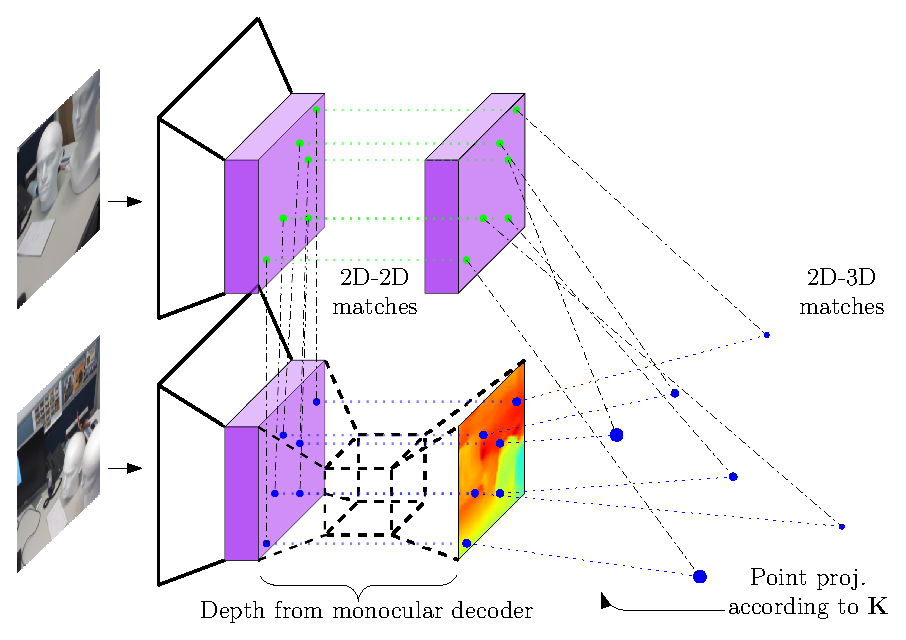
\includegraphics[width=0.9\linewidth]{method/pnlp.eps}}
    \end{minipage}\hfill
	\begin{minipage}{0.5\linewidth}
   		\subfigure[][IClP]{\label{fig:iclp}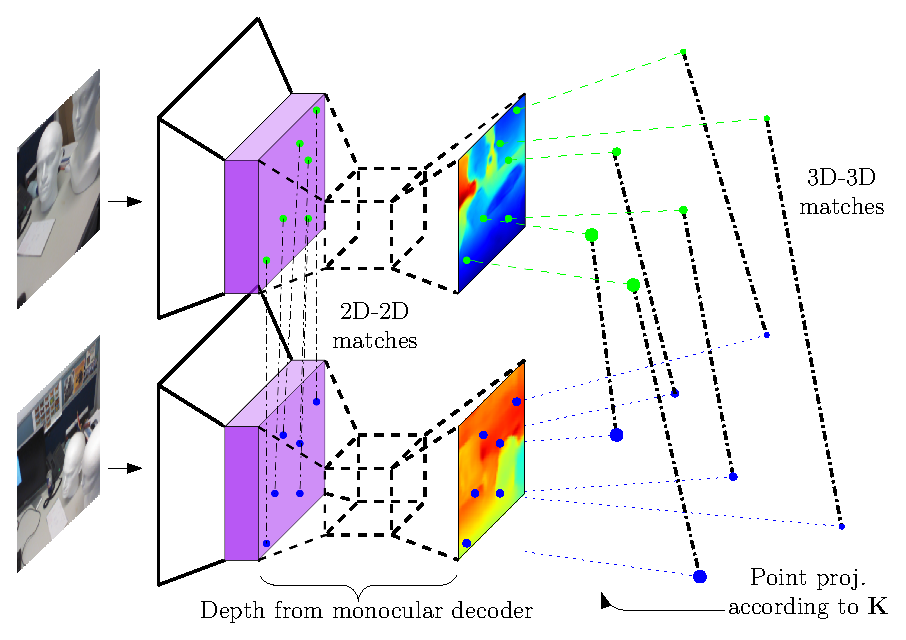
\includegraphics[width=0.9\linewidth]{method/iclp.eps}}
	\end{minipage}
	
	\caption[]{\textbf{:} \ref{fig:pnlp} \ref{fig:iclp} \label{fig:relative_pose}}
\end{figure}


\label{sec:relative_pose}
We propose two alternative to compute the relative pose between the query image $x^q$ and the most similar retrieved images $x^{sim}_j, j \in [1, K]$:
\begin{enumerate}
	\item an \ac{icp}-based method called \ac{iclp} see section~\ref{subsec:pc_alignment},
	\item a \ac{pnp}-based algorithm called \ac{pnlp}, see section~\ref{subsec:pnlp}.
\end{enumerate}
\noindent The main differences between these two approaches are that \ac{iclp} is iterative an rely on the reconstructed depth map of the two densely matched images, while \ac{pnlp} is using only one depth map. In figure~\ref{fig:relative_pose}, our two relative pose estimation are presented, side by side.

\subsection{Iterative Closest Learned Point}
\label{subsec:pc_alignment}
The general idea is to obtain the relative camera pose $\mathbf{h}^\mathrm{r \rightarrow q}$ by registering the point cloud $\mathcal{P}^q$ obtained by projecting in 3D the depth map (equation~\ref{eq:3d_proj}) $\hat{z}^q$ of query $x^q$ to the points cloud $\mathcal{P}^{sim}_j$ from the reference depth maps $\hat{z}^{sim}_j$ of images $x^{sim}_j, j \in [1, K]$. One reference point cloud is evaluate at a time and we chose the final registration that minimise the point-to-point distance between the two point clouds.

\begin{table}
\centering

\begin{minipage}{0.5\linewidth}
\centering

\begin{footnotesize}
\renewcommand{\arraystretch}{1.1}
\newcolumntype{C}[1]{>{\centering\arraybackslash}m{#1}}
\begin{tabular}{m{0.2\linewidth} | C{0.3\linewidth} C{0.3\linewidth}}
7 Scenes \citep{Shotton2013}  & \ac{iclp} w/o deep features & \ac{iclp} w/ deep features\\
%	\cline{3-8} 
	\hline
	\hline	
	Chess 	& $0.28/8.6$		&	$\mathbf{0.23/5.4}$	\\
	Fire	    &	$0.39/16.5$		& $\mathbf{0.30/14.1}$	\\
	Heads   &	$\mathbf{0.18}/14.9$	&	$0.19/\mathbf{14.1}$	\\
	Office   &	$0.41/13.4$	& $\mathbf{0.36/11.3}$	\\
	Pumpkin 	&	$0.40/12.0$	&	$\mathbf{0.35/7.4}$	\\
	Kitchen & 	$0.24/\ 7.5$	&	$\mathbf{0.19/4.9}$		\\
	Stairs  	&	$0.57/12.2$	&	$\mathbf{0.48/10.3}$	\\
	\hline
\end{tabular}
\end{footnotesize}

\end{minipage}\hfill
\begin{minipage}{0.5\linewidth}
\centering

\caption[Point cloud alignement]{\label{tab:methods_comparison}\textbf{Point cloud registration:} we report median error on position and orientation (m/$^{\circ}$) for each scene. Its shows the importance of deep feature for point cloud matching in our method. Global image descriptors for image indexing are \ac{mac} descriptor, see section~\ref{sec:implementation} for more details about the used datasets and our implementation.}

\end{minipage}

\end{table}
\paragraph{Point matching.}
\label{para:pc_matching}
Refinement with \ac{icp} involves matching corresponding points between two point clouds in order to estimate a rigid transformation that minimises the distances between the paired points. Standard approaches only consider the Euclidean distance between a single point and its nearest neighbours in the reference point cloud to establish matching, making the initial alignment between the two point clouds a crucial step to obtain correct results. We can rely on point descriptors to establish strongest matches~\cite{Pomerleau2015}. We use local descriptor $d_{l,m}$ introduced in section~\ref{subsec:matching} and we associate to each projected point $\mathbf{p}_{l,m}$ a the descriptor corresponding to the deep feature computed by the encoder $\mathrm{E}$ at the same spatial position $\left\{l,m\right\}$. The matching process remains the same as the one detailed in \S~\ref{subsec:matching}, with the additional 3D point information added to the local features. We present in table~\ref{tab:pc_alignment} results of an exploratory experiment to estimate the benefit of adding the deep features for the point cloud alignment. We observe a clear improvement at almost no cost (the deep features are extracted from the already computed features block of the depth from monocular \ac{cnn}).  

\begin{algorithm}
 \KwData{initial pose $\mathbf{h}_{init}$, point cloud to align $\mathcal{P}$ with associated descriptors $\mathcal{D}$ and reference point cloud $\mathcal{P}_{ref}$ with assocaited descriptors $\mathcal{D}_{ref}$}
 \KwResult{final pose $\mathbf{h}_{refined}$}
% initialization\;
 $\mathbf{h}_{refined} \gets \mathbf{h}_{init}$\;
 $\mathbf{h}_{relative} \gets \mathbf{1}_{4\times 4}$\;
 \While{$\norm{\mathbf{h}_{relative} - \mathbf{I}_{4\times 4}}_{\mathrm{F}} \geq \epsilon $}{
    $\mathcal{P}_{aligned} \gets \mathbf{h}_{refined}\mathcal{P}$\;
	$\mathcal{M} \gets \mathtt{match\_points}(\mathcal{P}_{aligned}, \mathcal{P}_{ref}, \mathcal{D}, \mathcal{D}_{ref})$\;  
	$\mathbf{h}_{relative} \gets \mathtt{relative\_pose}(\mathcal{M})$\;
    $\mathbf{h}_{refined} \gets \mathbf{h}_{relative}\mathbf{h}_{refined}$\;
 }
 \If{$\norm{\mathcal{M}}_2 > \epsilon_{repro}$}{
     $\mathbf{h}_{refined} \gets \mathbf{h}_{init}$\;
 }

 \caption{\label{alg:icp}Our ICP algorithm, see text for details about functions $\mathtt{match\_points}$ and $\mathtt{relative\_pose}$. Pose refinement is rejected if the mean distance between matched points, $\norm{\mathcal{M}}_2$, is superior to $\epsilon_{repro}$.}
\end{algorithm}
\paragraph{Algorithm.} \label{para:pc_alignment} Relative pose $\mathbf{h}^\mathrm{r \rightarrow q}$ is obtain thank to the iterative algorithm detailed in~\ref{alg:icp}. The $\mathtt{relative\_pose}$ function computes the relative transformation between the matched points that minimises the Euclidean difference between the two point clouds. We use classical relative pose estimation algorithm~\citep{Pomerleau2015}:  
\begin{itemize}
	\item Rotation: we use a \ac{svd} on the matching matrix obtained by multiplication of the zeros-centred corresponding 3D points in each point cloud. Rotation matrix can computed by multiplying the right-singular vectors matrix with the transposed of the left-singular vectors matrix.
	\item Translation: we obtain the translation component by aligning in the same frame the two point cloud centroids, using the rotation matrix, and evaluating the difference between them.
\end{itemize}

We embed the pose computation within a \ac{ransac}, as the point cloud may contain erroneous data because it has been generated from image-only information by our encoder/decoder. We run the algorithm for a fixed size of iterations, for each of the top $K$ retrieved images by the first indexing step. We chose the final relative pose $\mathbf{h}^\mathrm{r \rightarrow q}_{best}, best\in\left[1,K\right]$ according to the minimal mean alignment error returned by our algorithm ($\norm{\mathcal{M}}_2$).

\subsection{Perspective-n-learned-Points}
\label{subsec:pnlp}
Thanks to the generated depth map (section~\ref{subsec:depth_map}) and the equation~\ref{eq:3d_proj}, we can project 2D points from retrieved images into 3D coordinates. 2D-2D correspondences obtained in section~\ref{subsec:matching} can be interpreted as 2D-3D correspondences and we can use a \ac{pnp} algorithm to compute the relative transformation $\mathbf{h}_\mathrm{r \rightarrow q}$ between the query image and the reference image. 

We embed our \ac{pnlp} algorithm within a RANSAC consensus where a sub-part of 2D-3D correspondences are evaluated at a time. We use 3-points algorithm from~\citep{Kneip2011}, using the authors efficient implementation~\citep{Kneip2014opengv}. As we have $K$ reference candidates from image retrieval step (section~\ref{subsec:image_indexing}), we select the best pose $\mathbf{h}^\mathrm{r \rightarrow q}_{best}, best\in\left[1,K\right]$, with the largest proportion of inlier correspondences after the \ac{pnp} optimisation. If the ratio of inlier is below a given threshold, we simply affect the pose of the retrieved image to the query.

\subsection{Final pose computation}
We obtain final pose of query image $\mathrm{x^q}$ using the relation:
\begin{equation}
	\mathbf{h}^\mathrm{q} = \mathbf{h}^\mathrm{r}_{best}\mathbf{h}^\mathrm{r \rightarrow q}_{best}.
\end{equation}

\subsection{System design and motivation}
\paragraph{Multi-task model.} In order to make our system fast and lightweight, we use a single encoder/decoder neural network for the three tasks needed in our pose estimation pipeline. That means with a single image forward, we obtain a compact global image description, dense local descriptors and a depth map corresponding to the observed scene.

\paragraph{Single task training policy.} There are dedicated training pipeline for each of the computer vision tasks involved in our image pose estimation framework: methods for learning a global image descriptor~\citep{Arandjelovic2017, Radenovic2017, Gordo2017}, CNN designed to extract and describe local features~\citep{Yi2016a, Rocco2018, Ono2018} and system that produces a depth map from a monocular image~\citep{Eigen2014, Godard2017, Mahjourian2018}. We decide to train our encoder/decoder network for the task of depth from monocular estimation because estimation of erroneous depth measurement will result in wrong estimation of the final pose. In the next section, we experimentally show that even if our network has not been trained especially for the task of image description or local feature matching, the latent features computed within the network embed enough high-level semantic to perform well on these tasks~\citep{Taira2018, Zamir2018}.

\paragraph{Generalization.} Because we rely on a non-absolute representation of the scene geometry (depth is estimated \textit{relatively} to the camera frame), our model is not limited to localization on one specific scene like end-to-end pose estimation networks~\citep{Kendall2017, Brachmann2017b}. In other words, the same trained network can be used to localize images in multiple indoor and outdoor scenes, and even on totally unknown environments. 